\documentclass[11pt,letterpaper]{article}

% --- Packages ---
\usepackage[utf8]{inputenc}
\usepackage[T1]{fontenc}
\usepackage[margin=1in,top=1in,bottom=1in]{geometry}
\usepackage{graphicx}
\usepackage{xcolor}
\usepackage{hyperref}
\usepackage{booktabs}
\usepackage{tabularx}
\usepackage{array}
\usepackage{enumitem}
\usepackage{titlesec}
\usepackage{fancyhdr}
\usepackage{listings}
\usepackage{tikz}
\usepackage{caption}
\usepackage[final,protrusion=true,expansion=false]{microtype}
\usepackage{tocloft}
\usepackage{parskip}

\usetikzlibrary{shapes.geometric,arrows.meta,positioning,calc,backgrounds,fit}

% --- Paragraph style ---
\setlength{\parskip}{0.6em}
\setlength{\parindent}{0pt}

% --- Hyperref setup ---
\hypersetup{
    colorlinks=true,
    linkcolor=black,
    citecolor=black,
    urlcolor=blue!60!black,
    pdftitle={Sail Protocol Whitepaper},
    pdfauthor={Alejandro Dopico}
}

% --- Title formatting ---
\titleformat{\section}
  {\normalfont\Large\bfseries}{\thesection}{0.7em}{}
\titleformat{\subsection}
  {\normalfont\large\bfseries}{\thesubsection}{0.7em}{}
\titleformat{\subsubsection}
  {\normalfont\normalsize\bfseries}{\thesubsubsection}{0.6em}{}

\titlespacing{\section}{0pt}{1.6em}{0.7em}
\titlespacing{\subsection}{0pt}{1.2em}{0.4em}
\titlespacing{\subsubsection}{0pt}{1.0em}{0.3em}

% --- TOC dotted leaders ---
\renewcommand{\cftsecleader}{\cftdotfill{\cftdotsep}}

% --- Code listing style ---
\definecolor{codebg}{rgb}{0.97,0.97,0.97}
\definecolor{codecomment}{rgb}{0.5,0.5,0.5}
\definecolor{codekeyword}{rgb}{0.15,0.25,0.55}
\definecolor{codestring}{rgb}{0.5,0.1,0.1}
\definecolor{accent}{rgb}{0.32,0.18,0.12}
\definecolor{accentlight}{rgb}{0.94,0.91,0.88}

\lstdefinelanguage{Solidity}{
  keywords={pragma,solidity,contract,interface,abstract,function,external,internal,public,private,view,pure,returns,address,uint256,bytes32,bytes4,bool,bytes,calldata,memory,storage,if,else,for,while,return,emit,event,modifier,struct,enum,mapping,using,import,constructor,require,assert,revert,virtual,override,immutable,constant,this,new,delete,is},
  keywordstyle=\color{codekeyword}\bfseries,
  comment=[l]{//},
  morecomment=[s]{/*}{*/},
  commentstyle=\color{codecomment}\itshape,
  string=[b]",
  stringstyle=\color{codestring},
  sensitive=true,
  morestring=[b]'
}

\lstset{
  language=Solidity,
  basicstyle=\ttfamily\small,
  backgroundcolor=\color{codebg},
  frame=single,
  framerule=0pt,
  rulecolor=\color{codebg},
  xleftmargin=0.5em,
  xrightmargin=0.5em,
  framexleftmargin=0.5em,
  aboveskip=1em,
  belowskip=1em,
  showstringspaces=false,
  breaklines=true,
  numbers=none,
  captionpos=b
}

% --- Page style ---
\fancypagestyle{plain}{
  \fancyhf{}
  \renewcommand{\headrulewidth}{0pt}
  \fancyfoot[C]{\thepage}
}

\fancypagestyle{main}{
  \fancyhf{}
  \fancyhead[L]{\small\textit{Sail Protocol}}
  \fancyhead[R]{\small\textit{May 2026}}
  \fancyfoot[C]{\thepage}
  \renewcommand{\headrulewidth}{0.4pt}
}

% --- Custom commands ---
\newcommand{\code}[1]{\texttt{\small #1}}

% --- Document ---
\begin{document}

% --- Cover page ---
\pagestyle{plain}
\begin{titlepage}
\centering
\vspace*{1.5cm}


\includegraphics[width=0.18\textwidth]{sail_logo.png}

\vspace{1.5cm}

{\Huge\bfseries Sail Protocol\par}
\vspace{0.7cm}
{\LARGE\bfseries Onchain Separately Managed Accounts\\Run by Agents\par}

\vspace{1.5cm}

{\large Alejandro Dopico, Cofounder and CEO\par}
\vspace{0.3cm}
{\normalsize Contributors: Alvaro Alonso, Andrés Sarría, Samuel Schmitt\par}

\vspace{0.7cm}

{\normalsize May 2026\par}

\vfill

{\normalsize\ttfamily https://sail.money\par}

\end{titlepage}

% --- Abstract ---
\thispagestyle{plain}
\section*{Abstract}

The world is moving toward an agent economy. Autonomous software agents, built on large language models and other AI systems, are increasingly able to execute financial decisions at machine speed. To act on-chain on behalf of capital they do not own, agents need two properties at once: the ability to sign transactions, and enforceable bounds on what they may do. Existing approaches force a choice between them: give the agent a private key and surrender custody, or run the agent through an off-chain co-signer and lose machine speed.

Legal mandates, the substrate that governs traditional separately managed accounts (SMAs), cannot serve agents. An agent executing continuously cannot be governed by paperwork it cannot read. The bounds must be code, evaluated on every transaction, revocable in a single block.

Sail Protocol is the infrastructure for that relationship. The protocol formalizes the onchain SMA: a self-custodial account, held by the LP through a Safe, whose mandate is enforced by smart contracts on every manager transaction. Three roles are separated explicitly. The Owner holds the Safe. The Permission Signer authorizes the mandate. The Manager executes within bounds. The Manager is typically an agent.

Permissions are user-deployed Solidity contracts. The manager's signature names one registered permission as the authorizer for each dispatch; the kernel evaluates that permission via \code{staticcall} under a gas cap and dispatches the call to the Safe only if it returns \code{true}. Because permissions are arbitrary Solidity, any DeFi primitive can be a permission. The protocol covers, by construction, everything DeFi can do.

The protocol enforces two fee mechanisms: a per-permission registration fee paid to the protocol treasury, and a protocol cut on manager-collected fees. The protocol cut is set to zero at protocol launch. Anyone can deploy SMAs, write permissions, and operate as a manager.

The agent economy combined with onchain SMA infrastructure is the path to personalized portfolio management at any account size. The SMA structure has been the dominant primitive for personalized wealth management at the high end for a century. With code-enforced mandates and machine managers, that structure becomes feasible for anyone with a wallet.

Sail's mission is to unlock personalized finance for all.

\vspace{0.8cm}
\noindent\textbf{Keywords:} separately managed accounts, autonomous agents, account abstraction, Gnosis Safe, code-enforced mandates, DeFi, custody, permissions

\newpage

% --- Contents ---
\thispagestyle{plain}
\renewcommand{\contentsname}{\Large Contents}
\tableofcontents

\newpage
\pagestyle{main}

% --- 1. Introduction ---
\section{Introduction}

Personalized investment management has historically been an institutional product. A separately managed account (SMA) is the legal and operational structure that supports it: capital is held in an account titled to the owner, while a designated manager executes investments within bounds set by a mandate. Unlike pooled vehicles --- mutual funds, hedge funds, vault tokens --- the assets remain separately custodied for each client.

The SMA relationship has four properties that pooled vehicles cannot match. Capital remains under the owner's name and custody. The manager has bounded authority, not full discretion. The mandate can be revised, narrowed, or revoked at any time. Performance and risk are attributed per account, not blended.

These properties make the SMA the dominant primitive for serious capital. They have also kept SMAs inaccessible to most investors. Account minimums of \$100{,}000 to \$1{,}000{,}000 are typical. The operational cost of running a true SMA at smaller account sizes --- the custodian fees, the legal infrastructure, the reconciliation overhead --- is prohibitive.

\subsection{The Gap in Onchain Managed Accounts}

Decentralized finance has not yet replicated the SMA. The dominant managed-account pattern in DeFi today is the pooled vault: depositors mint shares of a strategy operated by a single manager. Vaults are powerful, but they are not SMAs. Depositors give up account-level custody to the vault contract, share performance attribution with every other depositor, and inherit the strategy's full risk profile rather than parameterizing their own bounds.

Self-custodial smart wallets --- including the broader account-abstraction family --- preserve custody but offer no native concept of a manager bounded by a mandate. They are wallets, not protocols for delegated execution.

The category between pooled vaults and bare smart wallets --- an onchain SMA primitive --- has been missing.

\subsection{Agents as the Forcing Function}

The need for an onchain SMA primitive has become urgent because of autonomous agents. AI systems can execute trades, rebalance portfolios, and respond to market conditions continuously. To do this onchain they require two things: the ability to sign transactions on behalf of capital they do not own, and enforceable bounds on what they may do.

Existing approaches resolve only one of these at a time. Giving an agent a private key surrenders custody. Running an agent off-chain with a co-signed multisig preserves custody but reintroduces the slowness and operational overhead that traditional SMAs already suffer from. Neither solution is satisfactory.

The SMA primitive resolves both at once. The agent is the Manager. The LP retains custody through a self-custodial Safe. The mandate --- what the agent may and may not do --- is enforced by smart contract code on every transaction. Replacing the legal mandate with a code-enforced mandate is the only mandate model that operates at machine speed. An agent cannot be governed by paperwork it cannot read.

\subsection{Agentic Dynamic Strategies}

The convergence of agent execution and code-enforced mandates enables a new class of investment approach: the agentic dynamic strategy.

Traditional investment mandates are static. A discretionary manager receives a risk profile and a set of constraints, then applies them uniformly across a book of accounts. The same template governs every client. Personalization happens at the margins --- a higher equity allocation here, a different duration target there --- but the underlying strategy is shared across many accounts.

An agent running within a Sail SMA operates differently. The mandate --- expressed as registered permissions --- sets the hard outer boundary of what the agent may do. Within that boundary, the agent constructs and executes a strategy that is continuously sensitive to the individual owner's parameters: current portfolio balance, risk tolerance, yield preferences, time horizon, liquidity needs, and the owner's broader utility function. These inputs are not fixed; they evolve as the owner's situation changes, and the agent adapts with them.

This makes genuine personalization possible at scale. In a pooled strategy, every depositor inherits the same allocation, the same timing, the same risk exposure. In an agent-run SMA, each account is fully separate. An agent managing a thousand accounts runs a thousand distinct strategies --- each calibrated to its owner --- while sharing the same protocol infrastructure, the same permission templates, and the same fee model. The marginal cost of serving one more account with a tailored strategy is the cost of one more agent execution.

Agentic dynamic strategies represent a new kind of asset management: not algorithmic trading (same logic applied uniformly to all) and not traditional private wealth management (too expensive per account to scale), but individually calibrated portfolio management made operationally feasible by autonomous agents and structurally feasible by the onchain SMA primitive.

\subsection{The Sail Thesis}

Sail Protocol provides the infrastructure to express the SMA relationship onchain. The core thesis is that the mandate substrate should be minimal: a trusted kernel that handles account instantiation, permission registration, manager dispatch, and fee splitting; everything else --- what permissions look like, how fees are calculated, how NAV is reported, which DeFi venues are supported --- should live in user-deployed contracts outside the trusted core.

The kernel is auditable in isolation. Each permission is auditable in isolation. The protocol can support any DeFi primitive without changing the kernel.

This design makes onchain SMAs cheap enough to operate at any account size. An autonomous agent serving an SMA holding \$1{,}000 incurs the same protocol cost as one serving an SMA holding \$1{,}000{,}000. The marginal cost of personalization, in protocol terms, is zero. That is what enables Sail's mission: \emph{personalized finance for all}, made operationally feasible by autonomous agents and structurally feasible by minimal infrastructure.

% --- 2. Problem Statement ---
\section{Problem Statement}

\subsection{Onchain SMA Requirements}

The SMA structure has six core requirements. An onchain SMA protocol must provide all of them.

\begin{enumerate}[leftmargin=1.5em,itemsep=4pt]
  \item \textbf{Self-custody.} The LP must retain custody of the capital at all times. Manager compromise must not result in loss of principal.
  \item \textbf{Bounded authority.} The manager must have authority to execute, but only within explicit bounds the owner has approved.
  \item \textbf{Granular enforcement.} Bounds must be enforceable at calldata level --- recipients, swap amounts, LTV ratios, slippage tolerances, allowed protocols --- not merely contract-level allowlists.
  \item \textbf{Deterministic settlement.} Manager fees must accrue and settle through onchain rules, not off-chain reconciliation.
  \item \textbf{Revocability.} The owner must be able to revoke manager authority at any time without manager cooperation.
  \item \textbf{Composability.} The SMA must integrate with existing DeFi infrastructure --- DEXes, lending markets, perpetual venues, restaking, RWA --- without requiring per-venue protocol changes.
\end{enumerate}

\subsection{Comparison of Existing Approaches}

Existing onchain managed-account approaches each cover some of these requirements but none cover all six.

\begin{table}[h]
\centering
\renewcommand{\arraystretch}{1.4}
\small
\begin{tabularx}{\textwidth}{@{}l X X X@{}}
\toprule
\textbf{Approach} & \textbf{Custody} & \textbf{Manager bounds} & \textbf{DeFi composability}\\
\midrule
Traditional SMA & Held by custodian & Legal mandate & Venue-bound\\
DeFi pooled vault & Pooled in contract & Strategy code & Venue-bound\\
Smart wallet alone & Self-custodial & Wallet roles only & Any\\
Off-chain co-signer & Self-custodial & Manual co-sign & Any, slow\\
\midrule
\textbf{Sail Protocol} & Self-custodial & Calldata-level permissions & Any\\
\bottomrule
\end{tabularx}
\caption{Onchain SMA requirements satisfied by approach.}
\end{table}

The Sail thesis is that all six requirements can be satisfied by a single protocol if the trusted core is kept narrow and the venue-specific complexity is pushed into composable, user-deployed contracts.

% --- 3. Protocol Model ---
\section{Protocol Model}

\subsection{Three Roles}

Sail separates three roles that exist implicitly in any managed-account structure.

\begin{table}[h]
\centering
\renewcommand{\arraystretch}{1.4}
\small
\begin{tabularx}{\textwidth}{@{}>{\bfseries}p{2.6cm} X X@{}}
\toprule
\textbf{Role} & \textbf{Authority} & \textbf{Held by}\\
\midrule
Owner & Holds the Safe. Custodies the SMA's capital. Always self-custodial. & The LP, who owns the Safe.\\
Permission Signer & Authorizes the mandate. Signs registration, configuration, and revocation of permissions via EIP-712. & The Owner, or a separate signing key or multisig.\\
Manager & Executes transactions within bounds. Cannot exceed what the registered permissions allow. & EOA, multisig, MPC wallet, or autonomous agent.\\
\bottomrule
\end{tabularx}
\caption{Core protocol roles.}
\end{table}

The role of \emph{transaction submitter} --- the address that pays gas and submits the manager's signed dispatch --- is intentionally not an authority role. Any address may submit a transaction; authority derives from the Manager's signature, the registered permissions, and the kernel's evaluation of those permissions. This makes the protocol natively compatible with relayers, paymasters, and ERC-4337 bundlers.

\subsection{The Mandate}

In Sail, the mandate is not a document. It is the set of permissions registered for an SMA --- contracts implementing \code{IPermission} that define what the Manager is authorized to do. The Safe is the account the mandate applies to; it is not itself part of the mandate.

When the Manager submits a transaction, the signature names one registered permission as the authorizer. The kernel calls \code{evaluate()} on that permission alone and dispatches the call to the Safe only if it returns \code{true}. Other registered permissions are not consulted during the dispatch.

The mandate is therefore enforceable at every transaction. If the manager attempts to swap to an unallowed router, transfer to an unallowed recipient, borrow above the configured LTV, or call any function outside the registered permission set, the transaction reverts before any state change occurs.

% --- 4. Architecture ---
\section{Architecture}

\subsection{Components}

The protocol comprises five components in the trusted core, plus a default fee policy and a starter set of example permission templates in the wider audit scope.

\begin{table}[h]
\centering
\renewcommand{\arraystretch}{1.35}
\small
\begin{tabularx}{\textwidth}{@{}p{4.2cm} X@{}}
\toprule
\textbf{Component} & \textbf{Role}\\
\midrule
\multicolumn{2}{l}{\textit{Trusted core}}\\
\code{SailKernel} & Account registration, permission registry, signature verification, manager dispatch via Safe modules, fee collection, principal tracking.\\
\code{SailGovernance} & Protocol parameter governance with a timelock, two-step transfer, emergency pause with auto-expiry, and trusted Safe factory and singleton allowlists.\\
\code{MandateFactory} & Untrusted UX orchestrator. Bundles permission configuration and registration into single transactions. Holds no protocol-level privileges.\\
\code{BaseSharedPermission} & Abstract base for shared multi-tenant permission templates. EIP-712 domain, per-account nonces, ECDSA and ERC-1271 signature verification.\\
Interfaces & \code{IPermission}, \code{IConfigurablePermission}, \code{IFeePolicy}, \code{IOracle}, \code{IBatchPermission}, \code{IPermissionIntrospection}, \code{IAgentIdentityResolver}.\\
\midrule
\multicolumn{2}{l}{\textit{Default policy and example templates}}\\
\code{StandardFeePolicy} & Reference fee policy: management fee on AUM, performance fee above high-water mark.\\
\code{Shared*Permission} & A starter set of example permission templates demonstrating the pattern across common DeFi primitives (see Section~\ref{sec:expressiveness}).\\
\bottomrule
\end{tabularx}
\caption{Protocol components.}
\label{tab:components}
\end{table}

The trusted core is what users must trust to use Sail at all. The default policy and example templates are what users must trust if they choose them; alternative policies and templates can be deployed by anyone without protocol-level changes.

\subsection{Request Flow}

Figure~\ref{fig:flow} illustrates the dispatch path for a manager transaction.

\begin{figure}[h]
\centering
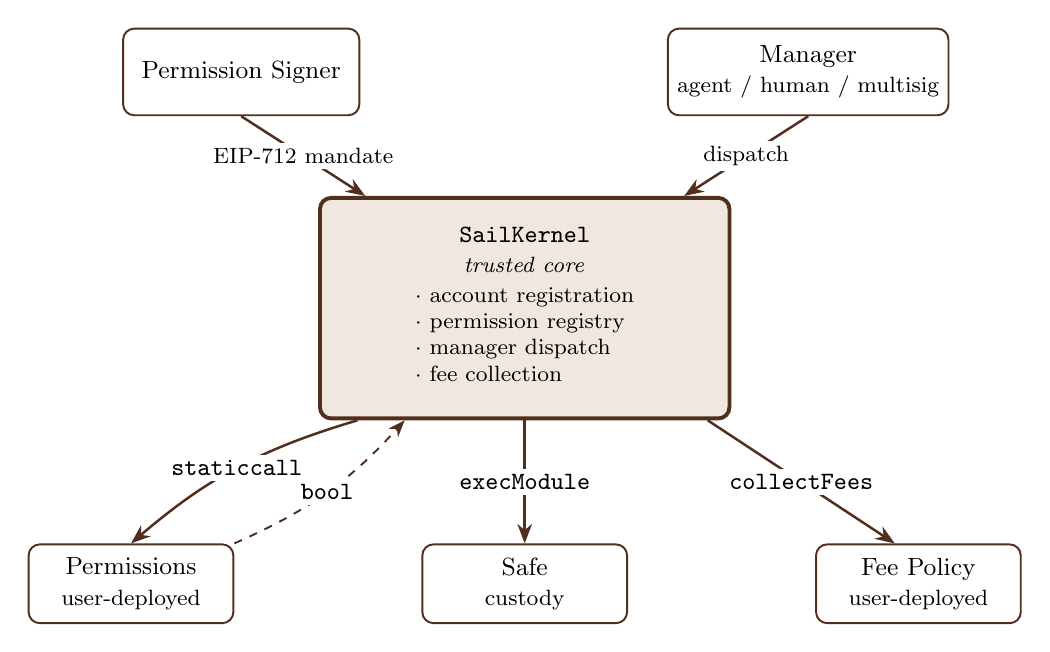
\begin{tikzpicture}[
  >=Stealth,
  every node/.style={font=\small},
  authoritybox/.style={
    rectangle, rounded corners=4pt,
    draw=accent, line width=0.7pt,
    minimum width=3.0cm, minimum height=1.1cm,
    align=center
  },
  kernelbox/.style={
    rectangle, rounded corners=4pt,
    draw=accent, line width=1.4pt,
    fill=accentlight,
    minimum width=5.2cm, minimum height=2.8cm,
    align=center
  },
  bottombox/.style={
    rectangle, rounded corners=4pt,
    draw=accent, line width=0.7pt,
    minimum width=2.6cm, minimum height=1.0cm,
    align=center
  },
  flowarrow/.style={->, thick, draw=accent, line width=0.9pt},
  returnarrow/.style={->, thick, draw=accent, line width=0.7pt, dashed}
]

% Top row - authority sources
\node[authoritybox] (signer) at (1.4, 0) {Permission Signer};
\node[authoritybox] (manager) at (8.6, 0) {Manager\\\footnotesize agent / human / multisig};

% Middle - kernel with internal responsibilities
\node[kernelbox] (kernel) at (5, -3) {%
  \textbf{\code{SailKernel}}\\
  \footnotesize\textit{trusted core}\\[3pt]
  \footnotesize\begin{tabular}{@{}l@{}}
    $\cdot$ account registration\\
    $\cdot$ permission registry\\
    $\cdot$ manager dispatch\\
    $\cdot$ fee collection
  \end{tabular}%
};

% Bottom row - three execution targets
\node[bottombox] (perms) at (0, -6.5) {Permissions\\\footnotesize user-deployed};
\node[bottombox] (safe) at (5, -6.5) {Safe\\\footnotesize custody};
\node[bottombox] (feepolicy) at (10, -6.5) {Fee Policy\\\footnotesize user-deployed};

% Authority arrows (top to kernel)
\draw[flowarrow] (signer.south) -- ($(kernel.north west)+(0.6,0)$)
  node[midway, fill=white, inner sep=2pt, font=\footnotesize]{EIP-712 mandate};
\draw[flowarrow] (manager.south) -- ($(kernel.north east)+(-0.6,0)$)
  node[midway, fill=white, inner sep=2pt, font=\footnotesize]{dispatch};

% Execution arrow + return: kernel <-> permissions (curved to avoid label overlap)
\draw[flowarrow] ($(kernel.south west)+(0.5,0)$) to[bend right=12]
  node[midway, fill=white, inner sep=2pt, font=\footnotesize]{\code{staticcall}}
  (perms.north);
\draw[returnarrow] (perms.north east) to[bend right=12]
  node[midway, fill=white, inner sep=2pt, font=\footnotesize]{\code{bool}}
  ($(kernel.south west)+(1.1,0)$);

% Execution arrow: kernel -> safe
\draw[flowarrow] (kernel.south) -- (safe.north)
  node[midway, fill=white, inner sep=2pt, font=\footnotesize]{\code{execModule}};

% Execution arrow: kernel -> fee policy
\draw[flowarrow] ($(kernel.south east)+(-0.3,0)$) -- ($(feepolicy.north)+(-0.3,0)$)
  node[midway, fill=white, inner sep=2pt, font=\footnotesize]{\code{collectFees}};

\end{tikzpicture}
\caption{Manager dispatch flow. The Permission Signer authorizes the mandate by EIP-712 signature. The Manager submits a transaction naming one registered permission as the authorizer. The kernel evaluates that permission via \code{staticcall}; if it returns \code{true}, the kernel forwards the call to the Safe through the Safe module interface. When the Manager calls \code{collectFees}, the kernel consults the registered Fee Policy and splits the result.}
\label{fig:flow}
\end{figure}

The kernel never holds custody of assets. The Safe holds the capital. The kernel holds only the permission list, principal accounting, and fee policy reference for each account.

\subsection{Batch Dispatch}

The protocol provides a second dispatch path for multi-step strategies that require atomic execution. \code{dispatchBatch()} accepts an ordered array of calls and a single batch permission --- a contract implementing \code{IBatchPermission} --- that validates the entire call sequence before any execution begins. Each call in the batch executes via the Safe module path in order; any subcall failure reverts the entire batch atomically.

This path is designed for DeFi strategies requiring temporary ERC20 approvals: the batch permission validates an approve-execute-reset sequence as a unit, enforcing that the approval amount matches the consumed amount and that the cleanup reset is present. It is equally available for any multi-step strategy where atomicity across calls is required.

The manager's signature commits to the permission address, the exact call array, a nonce, and a deadline. Batch dispatch follows the same selective authorization model as single dispatch: one named permission evaluates the entire batch, and other registered permissions are not consulted.

% --- 5. Permission System ---
\section{Permission System}

\subsection{The IPermission Interface}

A permission is a contract implementing a single interface:

\begin{lstlisting}
interface IPermission {
    function evaluate(bytes calldata txData, Context calldata ctx)
        external view returns (bool);
    function discriminator() external view returns (bytes32);
}

struct Context {
    address account;          // the Safe
    address manager;          // the delegated signer
    address submitter;        // msg.sender of dispatch (may be a relayer)
    address target;           // call target
    bytes4  selector;         // call selector
    uint256 value;            // msg.value
    uint256 blockTimestamp;
    uint256 blockNumber;
}
\end{lstlisting}

The \code{evaluate} function returns \code{true} if the transaction is allowed by this permission, \code{false} otherwise. The \code{discriminator} function returns a hash describing the (target, selector) tuple the permission gates, enabling the kernel to short-circuit irrelevant permissions for high-volume use cases.

\subsection{Evaluation Semantics}

The kernel's evaluation of registered permissions has four properties that together constitute the protocol's runtime guarantee.

\textbf{Static evaluation.} Permissions are called via \code{staticcall}, which prohibits state mutation. A permission cannot modify any contract's storage during evaluation. Reentrancy through the permission surface is structurally impossible.

\textbf{Gas isolation.} Each permission is called with a fixed gas cap. A permission that exceeds its cap reverts and is treated as returning \code{false}. A pathological permission cannot DoS the kernel or consume the manager's gas budget beyond the cap.

\textbf{Selective authorization.} The manager's signature names one registered permission as the authorizer for the dispatch. The kernel evaluates that permission alone --- no other registered permissions are consulted. The mandate is the union of registered permissions; each dispatch selects one as its authorizer. This enables multiple unrelated templates to coexist on one account: a swap permission, a borrow permission, and a transfer permission can all be registered, and each call selects the appropriate authorizer without the others falsely denying it. Batch dispatch follows the same model via the \code{IBatchPermission} interface.

\textbf{Fail-closed.} Any permission that reverts, runs out of gas, returns malformed data, or returns \code{false} causes the entire dispatch to revert. The default behavior of a buggy permission is to deny, not to allow.

\subsection{Full Expressiveness}
\label{sec:expressiveness}

Because permissions are arbitrary Solidity contracts, the protocol does not bound what a permission can express. Any DeFi primitive --- current or future --- can become a permission template by writing a contract. The protocol covers, by construction, the full surface of what DeFi can do.

This is a substantive design choice. The alternative path is a fixed-grammar mandate language: a set of enums describing conditions, references, parameter kinds, and value sources, interpreted by a constraint virtual machine inside the kernel. That approach trades expressiveness for predictability: the kernel knows exactly what every policy can do because the grammar is finite. The cost is that every new DeFi pattern --- a router with a new calldata shape, a yield protocol with a different reward structure, an emerging primitive that did not exist when the grammar was designed --- requires extending the grammar, updating the VM, and shipping a kernel upgrade.

Sail's approach inverts the trade-off. The kernel knows nothing about DeFi venues. It calls \code{evaluate()} on a permission contract and respects the answer. The structural guarantees (\code{staticcall}, gas cap, fail-closed, selective authorization) protect the kernel from the permission; everything the permission expresses inside that envelope is the author's responsibility, not the kernel's.

The result is that adding a new DeFi integration to Sail is a contract deployment, not a protocol upgrade. The kernel does not need to know about any specific DeFi venue --- existing or future. A permission contract that gates calls to a venue with the constraints its author chose is sufficient.

The single class of venues outside this expressiveness envelope is venues whose state is partly off-chain --- order books that match off-chain, settlement engines that sign off-chain. Permissions can constrain the on-chain boundary of such venues (deposits, withdrawals, allowed sub-accounts) but cannot constrain off-chain order signing. That is a property of those venues, not of the protocol.

\subsection{Example Templates}

To demonstrate the permission pattern across common DeFi primitives, Sail ships a starter set of example permission templates. Table~\ref{tab:templates} lists them.

\begin{table}[h]
\centering
\renewcommand{\arraystretch}{1.35}
\small
\begin{tabularx}{\textwidth}{@{}p{5.8cm} X@{}}
\toprule
\textbf{Template} & \textbf{Gates}\\
\midrule
\code{SharedBoundedSwapPermission} & AMM swaps. Router allowlist, token allowlist, per-transaction amount cap, optional oracle-based slippage check.\\
\code{SharedBoundedBorrowPermission} & Lending borrows. Protocol allowlist, asset allowlist, LTV check against an account collateral value oracle.\\
\code{SharedTransferTargetPermission} & ERC-20 transfers. Recipient allowlist, token allowlist.\\
\code{SharedDeFiBundlePermission} & Composite: swap, borrow, and transfer in one registered permission. Selector-routed evaluation.\\
\code{SharedPendlePermission} & Yield-protocol router: liquidity, principal-token swaps, yield-token swaps, mint/redeem, claim rewards.\\
\code{SharedAMMLiquidityPermission} & Concentrated liquidity operations on AMM position managers.\\
\code{SharedApproveAndCallBatchPermission} & Batch: atomic approve / protocol call / reset sequence. Enforces token allowlist, spender allowlist, amount cap, and mandatory reset to zero.\\
\bottomrule
\end{tabularx}
\caption{Example permission templates.}
\label{tab:templates}
\end{table}

These are not the protocol; they are demonstrations of the protocol. Anyone may deploy additional permission contracts for any DeFi venue. The kernel will register and dispatch through any contract that implements \code{IPermission}.

\subsection{Shared Multi-Tenant Templates}

The naive deployment pattern for permissions is one contract per account: each user deploys their own permission instance with their parameters in the constructor. This produces a clean per-instance audit surface but is expensive in gas and bytecode.

Sail's recommended pattern is the shared multi-tenant template. One contract is deployed once on each chain and serves every account that registers it. Per-account configuration is stored in mappings keyed by account address. Configuration is performed through \code{IConfigurablePermission}:

\begin{lstlisting}
interface IConfigurablePermission is IPermission {
    function configure(
        address account,
        bytes calldata params,
        uint256 deadline,
        bytes calldata sig
    ) external;
    function configureDirect(address account, bytes calldata params) external;
    function configNonces(address account) external view returns (uint256);
    function isConfigured(address account) external view returns (bool);
}
\end{lstlisting}

The \code{params} field is opaque template-specific calldata, decoded inside the template's configuration hook. The kernel and factory know nothing about \code{params}; new template shapes require zero changes to either.

\subsection{Permission Lifecycle}

A permission's lifecycle is governed by four operations, all authorized by the Permission Signer through EIP-712 signatures.

\textbf{Registration.} The Permission Signer signs a registration message containing the permission contract address. The kernel adds it to the account's permission list and charges the registration fee (Section~\ref{sec:fees}).

\textbf{Configuration.} For shared templates, the Permission Signer signs a configure instruction containing the template-specific params blob. Any caller may submit the signed call; the canonical orchestrator is the \code{MandateFactory}, but it holds no special privilege.

\textbf{Reconfiguration.} A subsequent \code{configure} call with a fresh nonce clears previous per-account state and applies the new params atomically.

\textbf{Revocation.} The Permission Signer signs \code{revokePermission}. The address is removed from the account's list. Two levels of revocation exist: revoking a single permission narrows the manager's authority; revoking the manager session entirely cuts off the manager.

\subsection{Optional Extension Interfaces}

Permission templates may optionally implement additional interfaces to expose metadata and capabilities to off-chain tooling, indexers, and the Sail Marketplace.

\textbf{IPermissionIntrospection.} Templates implementing this interface expose a stable identifier (\code{permissionId}), a version hash, a metadata URI, and an array of capability identifiers. The \code{SailCapabilities} library defines the canonical capability constants (\code{BOUNDED\_SWAP}, \code{BOUNDED\_BORROW}, \code{BATCH\_DISPATCH}, and others). Indexers use these to group accounts and dispatches by template type without maintaining a separate registry of known permission addresses. The Sail Marketplace uses capability identifiers for strategy discovery and filtering.

\textbf{IAgentIdentityResolver.} Templates operating under a known agent identity may implement this interface to expose an \code{AgentIdentityRef} associating the manager with an external identity registry, a chain, an agent ID, and a signing wallet. A per-account variant, \code{IAccountAgentIdentityResolver}, is available for shared templates where different accounts may be managed by different agents. This is metadata only --- the kernel does not read or verify agent identity. Identity-based authorization, if required, is enforced inside the template's own \code{evaluate()} implementation, not at the protocol level.

Neither interface is required by the kernel. Both are conventions for the template and tooling layer, consistent with Sail's design principle of keeping the trusted core minimal and pushing product-specific logic outward.

% --- 6. Fee Model ---
\section{Fee Model}
\label{sec:fees}

The protocol enforces two independent fee mechanisms. Each is capped by an immutable constitutional limit and tunable within that limit by governance.

\subsection{Fee 1: Permission Registration Fee}

When a permission is registered with the kernel, the registering account pays a flat ETH amount to the protocol treasury. The fee is identical regardless of contract size, deployment pattern, or template type.

\begin{quote}
\textit{total fee} = permissionRegistrationFee $\times$ $n_{\text{permissions}}$
\end{quote}

The storage variable \code{permissionRegistrationFee} is held in \code{SailGovernance}, bounded above by the immutable constitutional cap \code{MAX\_PERMISSION\_FEE\_WEI} = 0.001 ETH, and tunable by governance through a timelock. Excess \code{msg.value} on a registration call is refunded to the caller. The fee is denominated in native ETH and has no oracle dependency; governance is expected to retune the rate periodically as ETH price moves.

\subsection{Fee 2: Protocol Cut on Manager-Collected Fees}

When the Manager calls \code{collectFees}, the kernel asks the registered \code{IFeePolicy} for the legitimate fee amount, then splits it as follows:

\begin{quote}
\begin{tabular}{@{}l@{\;}c@{\;}l@{}}
\textit{protocol cut} & = & managerGrossFee $\times$ currentProtocolCutBps $/$ 10{,}000 \\
\textit{distributor cut} & = & (optional, defined by the fee policy) \\
\textit{manager take} & = & managerGrossFee $-$ protocol cut $-$ distributor cut
\end{tabular}
\end{quote}

The variable \code{currentProtocolCutBps} is governance-tunable, bounded above by an immutable constitutional cap. The constitutional cap is 25\% of manager-collected fees --- the protocol can never take more than a quarter of what a manager collects, regardless of any future governance procedure.

\textbf{The protocol cut is set to zero at protocol launch.} Fee 2 is built into the kernel built into the kernel but disabled by default; activation will be a separate governance decision tied to the readiness of the Sail Marketplace (Section~\ref{sec:marketplace}).

The kernel does not compute the gross fee. That responsibility lies in the registered \code{IFeePolicy} contract, which contains the schedule: management fee on AUM, performance fee on profits above high-water mark, hybrid models, or arbitrary custom math.

\subsection{Fee Policy Extensibility}

\code{IFeePolicy} is an interface, not a fixed contract. Sail ships with one reference implementation, \code{StandardFeePolicy}, which provides management fee on AUM and performance fee above a high-water mark. The reference policy uses a manager-attested NAV model: the manager reports the portfolio value at fee collection time. This is appropriate for self-managed SMAs where the manager and the LP are the same party (see Section~\ref{sec:trust}).

For third-party allocated strategies, alternative fee policy implementations will be needed. The Sail Marketplace roadmap (Section~\ref{sec:marketplace}) includes a spectrum of fee policy variants suited to different strategy archetypes: trustless NAV computed from on-chain position adapters for strategies that hold only verifiable positions; principal-bounded fees with performance crystallized only on withdrawal for high-turnover strategies where intermediate NAV is uncertain; independent attester co-signatures on NAV updates for strategies with mixed on-chain and off-chain positions.

None of these are part of the current audit scope. They are the work that follows once the Marketplace layer is built.

% --- 7. Governance ---
\section{Governance}

\subsection{Constitutional Caps}

Two constants are immutable in source code. No governance procedure can raise them.

\begin{itemize}[leftmargin=1.5em,itemsep=2pt]
  \item The maximum protocol cut on manager-collected fees: \code{MAX\_PROTOCOL\_CUT\_BPS} = 2{,}500 (25\%).
  \item The maximum permission registration fee: \code{MAX\_PERMISSION\_FEE\_WEI} = 0.001 ETH.
\end{itemize}

These bounds are not policy choices that governance enforces; they are properties of the deployed bytecode. A future governance under any control structure --- multisig, token, DAO, decision market --- cannot raise them. Lowering the active parameter inside these bounds remains possible.

\subsection{Governance Parameters}

The following parameters are mutable within the constitutional caps:

\begin{itemize}[leftmargin=1.5em,itemsep=2pt]
  \item The active protocol cut on manager-collected fees (default zero at launch).
  \item The active permission registration fee.
  \item Trusted Safe factory and singleton allowlists.
  \item Emergency admin (rotatable through the timelock).
\end{itemize}

Parameter mutations require a two-step process: a timelock delay followed by execution. Governance transfer is itself two-step (propose and accept). Emergency pause is a separate, lower-latency channel held by an emergency admin; pauses expire automatically and a cooldown applies between pause invocations to prevent denial of service by spam-pausing.

Governance is initially held by the team multisig. The contract is structured to support transfer to a token, DAO, or other mechanism without changes to the kernel.

% --- 8. Security Properties ---
\section{Security Properties}

\subsection{Formal Guarantees}

The protocol provides six formal guarantees, each a property of the deployed bytecode rather than of governance policy.

\begin{enumerate}[leftmargin=1.5em,itemsep=4pt]
  \item \textbf{Custody isolation.} The kernel cannot transfer Safe assets except through a manager dispatch that satisfies the named permission's evaluation. The kernel has no direct write access to the Safe outside the module dispatch path.
  \item \textbf{Selective authorization.} A manager dispatch succeeds only if the permission named in the manager's signature is registered for the account and returns \code{true} on evaluation. Other registered permissions are not evaluated during the dispatch.
  \item \textbf{Reentrancy safety.} Permission evaluation occurs via \code{staticcall}, which prohibits state mutation. No re-entry path exists through the permission surface.
  \item \textbf{Gas isolation.} Each permission is called with a fixed gas cap. A permission that exceeds its cap is treated as returning \code{false}; the kernel cannot be denied service by a malicious permission.
  \item \textbf{Constitutional fee caps.} Protocol cut and registration fee cannot exceed their constitutional bounds. No governance procedure can change this.
  \item \textbf{Signer separation.} The Permission Signer cannot move Safe assets. The Manager cannot register or revoke permissions. The Safe Owner can always revoke the Manager.
\end{enumerate}

\subsection{Known Limitations}
\label{sec:trust}

The protocol does not guarantee three properties that follow from its design as open infrastructure.

\textbf{Permission correctness.} A buggy permission is still a permission. The kernel verifies that a permission is a contract and that it returns \code{true} or \code{false}; it does not verify that the permission's logic correctly enforces what its author claims. Users are responsible for the permissions they register. The example templates will be externally audited; any other permission contract is at the user's own assessment.

\textbf{Manager-attested NAV.} The reference fee policy uses a manager-attested NAV model. A manager operating an SMA where a third party has deposited funds can in principle inflate the reported NAV when collecting fees. The maximum extractable amount is bounded by the Safe's liquid balance and the configured fee parameters but can reach a significant portion of the SMA's value in a single collection. This risk exists in any product built on Sail that uses the reference fee policy and accepts third-party LP deposits.

For this reason, Sail Protocol is designed for \emph{self-managed} SMAs --- developers, AI agent builders, and crypto-native users operating Safes with their own capital. In this configuration the trust model is irrelevant because the manager and the LP are the same party. The Sail Marketplace (Section~\ref{sec:marketplace}) is the curation layer that will introduce audited fee policy variants suited to third-party allocations.

\textbf{Off-chain venue components.} For DeFi venues whose state is partly off-chain --- venues with off-chain order books, venues with off-chain matching engines --- permissions can constrain the on-chain boundary (deposits, withdrawals, allowed sub-accounts) but cannot constrain the off-chain order signing. This is a property of those venues, not of Sail. Permissions for such venues must disclose which surfaces are enforced onchain and which inherit venue-specific trust assumptions.

% --- 9. Use Cases ---
\section{Use Cases}

The protocol is intentionally venue-agnostic. Any on-chain primitive becomes a permission template: AMM swaps, lending deposits and borrows and withdrawals, LP positions, perpetual trades, restaking deposits, prediction market bets, RWA flows. The example templates demonstrate the pattern across common DeFi primitives; additional templates for any DeFi venue can be deployed without protocol changes.

\subsection{Fully On-Chain Venues}

For venues with fully on-chain state --- spot AMMs, lending protocols, vault tokens, restaking primitives, on-chain options, on-chain prediction markets, RWA tokenizers --- permissions can enforce the full set of mandate constraints. Allowlisted routers, bounded swap amounts, LTV ceilings, slippage tolerances, recipient checks, and protocol allowlists are enforced at calldata level before the call leaves the kernel.

\subsection{Hybrid Venues}

For venues with mixed on-chain and off-chain state, permissions enforce only what is enforceable onchain. A permission for a venue with an off-chain order book, for example, can constrain bridge deposits, withdrawal recipients, and sub-account targets, but cannot constrain off-chain order signing. The boundary is documented per template; integrators building user-facing applications on Sail must surface these distinctions to LPs.

\subsection{Agent-Operated Strategies}

The dominant use case at launch is agent-operated SMAs. A developer building an AI agent strategy deploys a Safe, registers the permission templates corresponding to the agent's expected actions (swap, borrow, LP, claim), configures bounds (token allowlists, amount caps, LTV ceilings), and grants the agent's signing key as the Manager. The agent then runs continuously, executing whatever strategy it implements within the registered bounds. The agent cannot drain the Safe, cannot redirect funds, and cannot exceed its mandate. If the agent malfunctions or is compromised, the LP revokes its permissions onchain and the agent's authority ends immediately.

This is what makes the protocol useful as developer infrastructure for agent builders: the custody and bounds infrastructure is the protocol's responsibility, not the application's.

% --- 10. Personalized Finance for All ---
\section{Personalized Finance for All}
\label{sec:marketplace}

The path to broad accessibility has two stages.

\subsection{Stage 1: Protocol Infrastructure}

At launch, Sail serves developers, AI agent builders, and crypto-native users who deploy and operate their own SMAs. The Manager and the Owner are typically the same party: the user is running their own strategy, automated by their own agent or executed by their own hand. The protocol's role in this configuration is to provide custody-preserving execution and granular bounds for the user's own agent.

At protocol launch the protocol cut on manager-collected fees is set to zero. Managers operating their own SMAs at this stage pay only the per-permission registration fee, which is bounded by the constitutional cap and tunable within it by governance.

This stage is where the protocol earns its audit and stress-tests its assumptions. It is also where the agent-building developer community can be served immediately: an agent builder gets a complete custody substrate without designing and auditing one themselves.

\subsection{Stage 2: Sail Marketplace}

The Sail Marketplace, a forthcoming curation layer, will allow third-party managers to offer strategies to LPs who do not personally run an agent. The Marketplace will provide audited fee policy templates with explicit LP-protection guarantees suited to different strategy archetypes; curated manager discovery; risk parameter standardization across listed strategies; and distribution rails for allocators who want to allocate across multiple managers.

Managers listed on the Marketplace will be required to disclose, before any LP allocates capital to their strategy:

\begin{itemize}[leftmargin=1.5em,itemsep=2pt]
  \item Their active fee rates (management fee on AUM, performance fee on profits above HWM, any additional schedules).
  \item The specific \code{IFeePolicy} implementation governing their fee collection, and the audited trust model of that policy.
\end{itemize}

Marketplace listings will be expected to make these disclosures legible to LPs without requiring contract-level inspection.

The protocol cut on manager-collected fees may be activated by governance to accompany the Marketplace launch, providing revenue for the curation, audit, and distribution infrastructure. Until and unless the protocol cut is activated, managers retain the full fee amount their fee policy collects.

Until the Marketplace launches, third-party LP allocations on the open protocol carry the trust risk described in Section~\ref{sec:trust} and should not be made without independent due diligence on the manager, the fee policy, and the registered permissions.

\subsection{The Long-Term Vision}

The combination of three properties --- low operational cost (a minimal kernel with no per-account custodian), composable strategy expression (any DeFi venue becomes a permission template), and machine-managed execution (autonomous agents at any account size) --- makes the SMA structure feasible at the long tail of capital. A personalized portfolio strategy at \$1{,}000 has the same operational structure as the same strategy at \$1{,}000{,}000. The marginal cost of personalization, in protocol terms, is zero.

This is what we mean by \emph{personalized finance for all}. Not a single algorithm applied uniformly to everyone, but the SMA structure --- bounded, custody-preserving, mandate-driven, personalized to each owner --- made cheap enough to run for anyone with a wallet.

The personalized SMA has been the dominant primitive at the top of the wealth pyramid for a century. Sail is the infrastructure to extend it to everyone else.

% --- 11. Non-Goals ---
\section{Non-Goals}

Sail's design is shaped as much by what it excludes as by what it includes. The protocol explicitly does not provide:

\begin{itemize}[leftmargin=1.5em,itemsep=4pt]
  \item \textbf{Policy authoring workflow.} Drafts, versions, curation, subject access lists. Off-chain authoring --- Git, IDEs, SDKs, frontends --- handles this. The protocol stores deployed permission addresses, not authoring metadata.
  \item \textbf{A constraint grammar.} Solidity inside permission contracts replaces interpreted constraint structs. There is no enum of conditions, no grammar of references, no VM of operations. There is only the \code{IPermission} interface.
  \item \textbf{Workflow execution as a kernel concept.} A multi-step workflow is just a kind of permission: ``the transaction must conform to this shape.'' The protocol does not need to know.
  \item \textbf{ERC-4337 and EIP-7702 adapters in the kernel.} Peripheral adapter contracts wrap the kernel for users who want those entry points. The kernel remains transport-agnostic.
  \item \textbf{NAV computation.} Lives in user-deployed valuation modules and oracle adapters. Oracle choice is an ecosystem concern, not a protocol concern.
  \item \textbf{A registry of curators or template authors.} A Marketplace function, handled off-chain.
  \item \textbf{Identity primitives.} Permission modules may consult external identity registries; the kernel stays agnostic.
\end{itemize}

Each exclusion reduces what the protocol owns. The kernel owns less, by design, so that what it does own is provable, auditable, and stable for years.

% --- 12. Conclusion ---
\section{Conclusion}

Sail Protocol expresses the separately managed account relationship as a minimal onchain primitive. A small trusted kernel mediates between an Owner who holds custody through a Safe, a Permission Signer who authorizes the mandate, and a Manager who executes within bounds. Permissions are user-deployed Solidity contracts evaluated under structural safety guarantees --- \code{staticcall}, gas cap, selective authorization, fail-closed. Fees split through a protocol-enforced mechanism with an immutable constitutional cap. Anything beyond the kernel lives outside it: NAV, fee schedules, venue-specific gating, oracle policy.

The protocol exists because autonomous agents have made the legal mandate insufficient. An agent executing at machine speed cannot be governed by paperwork. The mandate must be code, evaluated on every transaction, revocable in a single block.

The protocol also exists because the SMA structure has been inaccessible to most investors for a century. The economics of running a custodian-mediated SMA do not work below institutional minimums. Onchain, with a minimal kernel and machine managers, the same structure can be operated at any account size. Personalized portfolio management becomes a primitive instead of a privilege.

The agent economy is the medium. The onchain SMA is the structure. Personalized finance for all is the destination.

\newpage

% --- Appendix A: Glossary ---
\section*{Appendix A: Glossary}
\addcontentsline{toc}{section}{Appendix A: Glossary}

\renewcommand{\arraystretch}{1.35}
\begin{tabularx}{\textwidth}{@{}p{4.0cm} X@{}}
\toprule
\textbf{Term} & \textbf{Meaning}\\
\midrule
Onchain SMA & A self-custodial managed account whose mandate is enforced by smart contract code on every transaction.\\
Mandate & The set of permissions registered for an SMA. Defines what the Manager is authorized to do. Enforced on every dispatch by the kernel's evaluation of the named permission.\\
Owner & The party who holds the Safe and owns the SMA's assets.\\
Permission Signer & The signer authorized to register, configure, and revoke permissions on the account. May be the same party as the Owner.\\
Manager & The party authorized to execute transactions on behalf of the account, within the bounds of the registered permissions. Typically an autonomous agent.\\
Permission & A Solidity contract implementing \code{IPermission}. An individual rule within an account's mandate. The kernel evaluates the permission named by the manager's signature for each dispatch.\\
Template & An example or reusable pattern for building a Permission. Sail ships a starter set of templates demonstrating the pattern across common DeFi primitives; anyone may deploy additional templates.\\
Batch permission & A Solidity contract implementing \code{IBatchPermission}. Validates an entire ordered call sequence before the kernel executes it atomically via \code{dispatchBatch()}.\\
Shared template & A Template implemented as a single permission contract that serves multiple accounts via per-account configuration storage; the recommended deployment pattern.\\
Fee 1 & Permission registration fee. Flat ETH per registered permission, paid to the protocol treasury.\\
Fee 2 & Protocol cut on manager-collected fees. Capped by the constitution. Set to zero at protocol launch.\\
Constitutional cap & A bound encoded in immutable source. No governance procedure can raise it.\\
Sail Marketplace & The forthcoming curation layer providing audited fee policies, manager discovery, and LP-protection guarantees for third-party allocations.\\
Selective authorization & The dispatch model in which the manager's signature names one registered permission as the authorizer; the kernel evaluates that permission alone.\\
Capability identifier & A \code{bytes32} constant from \code{SailCapabilities} that a template declares via \code{IPermissionIntrospection} to signal its functional capabilities to consumers.\\
\bottomrule
\end{tabularx}

\vfill

\rule{\textwidth}{0.4pt}\\
\small This document describes Sail Protocol, May 2026. The protocol has not been externally audited and is not deployed on mainnet. Information in this document is provided for technical evaluation. Nothing herein constitutes investment advice, an offer to sell, or a solicitation to buy any security or asset.

\end{document}
